\documentclass{ctexart}
% \usepackage[UTF-8]{ctex}
\usepackage{amsmath}
\usepackage{booktabs}
\usepackage{multirow}
\usepackage{tabularx}

\usepackage{booktabs,multirow,longtable}

\usepackage{listings}
\usepackage{color}

% 插入Matlab代码设置
\usepackage[framed, numbered, autolinebreaks, useliterate]{mcode}

%导言区插入下面三行
\usepackage{graphicx} %插入图片的宏包
\usepackage{float} %设置图片浮动位置的宏包
\usepackage{subfigure} %插入多图时用子图显示的宏包

% % 参考文献
% % 注意参考文献请用Biber编译,不能使用BiberTex或者BiberTex-8
\usepackage[backend=biber,style=gb7714-2015]{biblatex}
\addbibresource[location=local]{bib/sample.bib}

%% 引用网页
\usepackage{url}


% \definecolor{dkgreen}{rgb}{0,0.6,0}
% \definecolor{gray}{rgb}{0.5,0.5,0.5}
% \definecolor{mauve}{rgb}{0.58,0,0.82}

% \lstset{frame=tb,
%   language=Matlab,
%   aboveskip=3mm,
%   belowskip=3mm,
%   showstringspaces=false,
%   columns=flexible,
%   basicstyle={\small\ttfamily},
%   numbers=left,
%   numberstyle=\tiny\color{gray},
%   keywordstyle=\color{blue},
%   commentstyle=\color{dkgreen},
%   stringstyle=\color{mauve},
%   breaklines=true,
%   breakatwhitespace=true,
%   tabsize=3
% }



\title{CR-P0方法求解二维Stokes方程}
\author{谢文进}
\date{\today}
\begin{document}
\maketitle
\section{理论推导}
\subsection{问题描述}
对于Stokes问题
\begin{equation}
    \label{stokes}
    \left\{\begin{matrix}
        - \nu \Delta \mathbf{u}  + \nabla p = f, \quad \text{in } \Omega\\ 
        \nabla \cdot \mathbf{u} = 0 = h, \quad \text{in } \Omega \\
        \mathbf{u} = g = 0, \quad \text{on } \partial \Omega
    \end{matrix}\right.
\end{equation}
其中,取$\nu = 1$。这里函数$h(\mathbf{x},t)$为预留函数接口,方便后续处理随机项。

方程\ref{stokes}的弱形式为:找到$(\mathbf{u},p) \in  \mathbf{H}_0^1{(\Omega)} \times L_0^2{(\Omega)}$使得
\begin{equation}
    \label{weakStokes}
    \left\{\begin{matrix}
        a(\mathbf{u,v})+b(\mathbf{v},p)=(f,\mathbf{v}) \quad \forall \mathbf{v}\in \mathbf{H}_0^1{(\Omega)},\\ 
        b(\mathbf{u},q) = 0 = (h,q) \quad \forall q \in  L_0^2{(\Omega)},
    \end{matrix}\right.
\end{equation}
其中
$$
a(\mathbf{u,v})=\nu(\nabla \mathbf{u},\nabla \mathbf{v}), 
\quad b(\mathbf{v},p)=-(\text{div } \mathbf{v},p)
$$
对于二维情况,即找到$u_1\in H_0^1(\Omega)$,$u_2\in H_0^1(\Omega)$,
以及$p\in L_0^2(\Omega)$使得对$\forall v_1\in H_0^1(\Omega) $,
,$\forall v_2\in H_0^1(\Omega)$, $\forall q\in L_0^2(\Omega)$有下式\cite{FEM-何晓明}成立:
\begin{gather*}
    \label{weakStokes2}
        \int_{\Omega}\nu(2\frac{\partial u_1}{\partial x}\frac{\partial v_1}{\partial x}  +
        2\frac{\partial u_1}{\partial x}\frac{\partial v_1}{\partial x} +
        \frac{\partial u_1}{\partial x}\frac{\partial v_1}{\partial x} + 
        \frac{\partial u_1}{\partial x}\frac{\partial v_1}{\partial x} + 
        \frac{\partial u_1}{\partial x}\frac{\partial v_1}{\partial x} + \\
        \frac{\partial u_1}{\partial x}\frac{\partial v_1}{\partial x})dxdy 
        - \int_{\Omega}(p\frac{\partial v_1}{\partial x}
        + p\frac{\partial v_2}{\partial y})dxdy
        = \int_{\Omega}(f_1v_1+f_2v_2)dxdy,\\ 
        - \int_{\Omega}(q\frac{\partial u_1}{\partial x}
        + q\frac{\partial u_2}{\partial y})dxdy = 0
        =\int_{\Omega}hqdxdy.
\end{gather*}

\subsection{Crouzeix-Raviart三角形元\cite{有限元方法的数学基础}}
为方便计算,采用面积坐标$\lambda_i(\mathbf{x}),i=1,2,3$,$\lambda_i = \frac{S_i}{S}$。
Crouzeix-Raviart三角形元选取的是三边中点,
如图\ref{Fig.barycentric},可以得到基函数为

\begin{figure}[H] %H为当前位置,!htb为忽略美学标准,htbp为浮动图形
    \centering %图片居中
    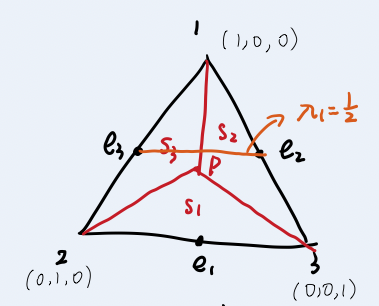
\includegraphics[width=0.7\textwidth]{img/barycentric.png} %插入图片,[]中设置图片大小,{}中是图片文件名
    \caption{Crouzeix-Raviart三角形元} %最终文档中希望显示的图片标题
    \label{Fig.barycentric} %用于文内引用的标签
\end{figure}

\begin{gather}
    \varphi_1 = -2(\lambda_1 - \frac{1}{2}), \\
    \varphi_2 = -2(\lambda_2 - \frac{1}{2}), \\
    \varphi_3 = -2(\lambda_3 - \frac{1}{2}).
\end{gather}
对上述基函数求梯度得:
\begin{equation}
    \label{基函数梯度}
    \frac{\partial \varphi_i}{\partial \lambda_j}=
    \left\{\begin{matrix}
        -2, \quad i=j,\\ 
        0, \quad i \neq j.
    \end{matrix}\right.
\end{equation}

\subsection{记号说明}
在推导离散格式之前,一些记号及编程数据结构说明
\cite{FEMCode}如下:
\begin{itemize}
    \item elem2dof:在边上点的全局坐标
    \item edge:边
    \item NE:边的个数
    \item NT:单元个数
    \item Nu:速度$u$的个数
    \item Np:压力$p$的个数
    \item N:顶点的个数
\end{itemize}

\subsection{有限元离散}
为了能够由数值实验进行计算,需要考虑有限元空间$\mathbf{U}_0^h \subset \mathbf{H}_0^1(\Omega)$及
$W_0^h \subset L_0^2(\Omega)$,即找到$\mathbf{u}_h \in \mathbf{U}_0^h$ 及
$p_h \in W_0^h$,使得对$\forall \mathbf{v}_h \in \mathbf{U}_0^h$ 及 $q_h \in W_0^h$ 有
\begin{gather*}
    a(\mathbf{u}_h,\mathbf{v}_h)+b(\mathbf{v}_h,p_h)=(f,\mathbf{v}_h),\\
    b(\mathbf{u}_h,q_h) =0= (h,q_h).
\end{gather*}
这里选取$U_h=span\{\phi _j\}_{j=1}^{N_u}$,$W_h=span\{\psi _j\}_{j=1}^{N_p}$,
$N_u$表示$\mathbf{u}_h$离散节点个数,$N_p$表示$p_h$离散节点个数。$\phi _j$由Crouzeix-Raviart
三角形元基函数确定,$\psi _j$为$P_0$多项式。

参考\citet{FEM程序理论},下面推导刚度矩阵及载荷向量:
\begin{gather*}
    a(\mathbf{u}_h,\mathbf{v}_h)=a(\sum_{i}\mathbf{u} _i \phi_i, \sum_j\mathbf{v}_j\phi_j ) = \sum_{i,j}a(\phi_i,\phi_j)
    \mathbf{u}_i\mathbf{v}_j=\mathbf{v}^T\mathbf{Au},\\
    b(\mathbf{v}_h,p_h)= b(\sum_{j}\mathbf{v} _j \phi_j, \sum_ip_i\psi_i ) = \sum_{i,j}b(\phi_j,\psi_i)\mathbf{v}_jp_i\\
=[\sum_{i,j}b(\phi_i,\psi_j)\mathbf{v}_ip_j]^T
=[\mathbf{p^TBv}]^T=\mathbf{v^TB^Tp},\\
(f,\mathbf{v}_h)=(\sum_if_i,\sum_j\mathbf{v}_j\phi_j)
=\sum_{i,j}(f_i,\phi_j)\mathbf{v}_j
=\mathbf{v^Tf},\\
b(\mathbf{u}_h,q_h)= b(\sum_{i}\mathbf{u} _i \phi_i, \sum_jq_j\psi_j ) 
= \sum_{i,j}b(\phi_i,\psi_j)\mathbf{u}_iq_j
=\mathbf{q^TBu},\\
(h,q_h)=(\sum_ih_i,\sum_jq_j\psi_j)
=\sum_{i,j}(h_i,\psi_j)q_j
=\mathbf{q^Th}.
\end{gather*}
写成矩阵形式,即为:
$$
\begin{pmatrix}
    \mathbf{v^T}   
    & \mathbf{q^T} 
    \end{pmatrix}
    \begin{pmatrix}
      \mathbf{A} &  \mathbf{B^T} \\
      \mathbf{B} & \mathbf{O} 
    \end{pmatrix}
    \begin{pmatrix}
     \mathbf{u} \\
    \mathbf{p} 
    \end{pmatrix}=
    \begin{pmatrix}
    \mathbf{v^T}   
    & \mathbf{q^T} 
    \end{pmatrix}
    \begin{pmatrix}
     \mathbf{f}\\
    \mathbf{h } 
    \end{pmatrix},
$$
则数值计算要求解的线性系统为
\begin{equation}
    \begin{pmatrix}
        \mathbf{A} &  \mathbf{B^T} \\
        \mathbf{B} & \mathbf{O} 
      \end{pmatrix}
      \begin{pmatrix}
       \mathbf{u} \\
      \mathbf{p} 
      \end{pmatrix}=
      \begin{pmatrix}
        \mathbf{f}\\
       \mathbf{h } 
       \end{pmatrix}.   
\end{equation}
\subsection{Dirichlet边界处理}
找到Dirichlet边界点,使得在这些点满足
$$
\mathbf{u}_i= g_i=0,
$$
对于Dirichlet边界条件$g(\mathbf{x},t)$,在程序中需要修正
矩阵$\mathbf{A}$,$\mathbf{B}$及右端项
$\mathbf{f}$,$\mathbf{h}$。

\section{数值实现}

\subsection{数值实例}
取$\Omega = [0,1]\times [0, 1]$,Stokes方程如下:
\begin{equation}
    \label{NumericalStokes}
    \left\{\begin{matrix}
        - \Delta \mathbf{u}  + \nabla p = \mathbf{f}, \quad \text{in } \Omega\\ 
        \nabla \cdot \mathbf{u} = 0 = h, \quad \text{in } \Omega \\
        \mathbf{u} = 0, \quad \text{on } \partial \Omega
    \end{matrix}\right.
\end{equation}
其中
\begin{gather*}
    f_1 = 2^{10}[(1-6x+6x^2)(y-3y^2+2y^3)+(x^2-2x^3+x^4)(-3+6y)\\
    -(-3+6x)(y^2-2y^3+y^4)],\\
    f_2 = -2^{10}[(-3+6x)(y^2-2y^3+y^4)+(x-3x^2+2x^3)(1-6y+6y^2)\\
    +(1-6x+6x^2)(y-3y^2+2y^3)].
\end{gather*}
方程\ref{NumericalStokes}的精确解为:
\begin{gather*}
    u_1 = -2^8(x^2-2x^3+x^4)(2y-6y^2+4y^3),\\
    u_2 = 2^8(2x-6x^2+4x^3)(y^2-2y^3+y^4),\\
    p = -2^8(2-12x+12x^2)(y^2-2y^3+y^4).
\end{gather*}
\subsection{重心坐标}
计算重心坐标的梯度\cite{FEMCode}
\begin{equation}
    \nabla \lambda_i = \frac{1}{2!|\tau|} \mathbf{n}_i
\end{equation}
其中$|\tau|$为三角形面积,在程序中$\nabla \lambda_i$为\mcode{Dlambda}。

下面推导计算三角形面积$|\tau|$,程序中变量名为\mcode{area},记$\mathbf{l}_i=\mathbf{x}_{i+1}-\mathbf{x}_{i-1}$,而
$\mathbf{n}_i=\mathbf{l}_i^{\bot}$,其中对于一个向量$\mathbf{v}=(x,y)$,
$\mathbf{v}^{\bot}=(-y,x)$。
对于三角形$T$,如图\ref{Fig.三角形},记$A_i=(x_i,y_i),i=1,2,3$。
\begin{figure}[H] %H为当前位置,!htb为忽略美学标准,htbp为浮动图形
    \centering %图片居中
    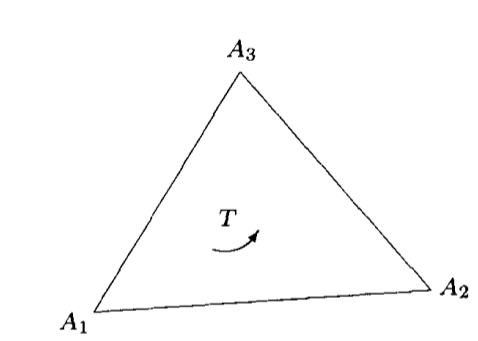
\includegraphics[width=0.7\textwidth]{img/三角元.png} %插入图片,[]中设置图片大小,{}中是图片文件名
    \caption{三角形} %最终文档中希望显示的图片标题
    \label{Fig.三角形} %用于文内引用的标签
\end{figure}
该三角形面积为
$$
|\tau|=\frac{1}{2}\left | \begin{matrix}
    x_1& y_1 & 1\\
    x_2& y_2 & 1\\
    x_3& y_3 & 1
  \end{matrix} \right |  
$$
而
$$
l_1=\begin{pmatrix}
    x_2-x_3\\
   y_2-y_3
   \end{pmatrix},
   l_2=\begin{pmatrix}
    x_3-x_1\\
   y_3-y_1
   \end{pmatrix},
   l_3=\begin{pmatrix}
    x_1-x_2\\
   y_1-y_2
   \end{pmatrix},
$$
经计算得到
\begin{gather*}
    -l_{31}l_{22}+l_{32}l_{21}=-(x_1-x_2)(y_3-y_1)+(y_1-y_2)(x_3-x_1)\\
=-(x_1y_3-x_1y_1-x_2y_3+x_2y_1)+(x_3y_1-x_1y_1-x_3y_2+x_1y_2)\\
=(x_2y_3-x_3y_2)-(x_1y_3-x_3y_1)+(x_1y_2-x_2y_1)\\
=\left | \begin{matrix}
    x_1& y_1 & 1\\
    x_2& y_2 & 1\\
    x_3& y_3 & 1
  \end{matrix} \right |,
\end{gather*}
因此
$$
|\tau|=\frac{1}{2}(-l_{31}l_{22}+l_{32}l_{21})
$$

关于该部分的计算代码见\mcode{gradbasis.m}\cite{iFEM}。
\subsection{Laplace算子}
下面推导如何生成矩阵$\mathbf{A}$,由前述理论推导知
\begin{gather*}
    \mathbf{A}_{ij}=a(\phi_i,\phi_j)=(\nabla \phi_i,\nabla \phi_j)
    =\iint\nabla \phi_i \cdot \nabla \phi_jdxdy\\
    =\iint-2\nabla \lambda _i\cdot (-2\nabla \lambda _j)dxdy
    = 4 |\tau |\nabla \lambda _i\cdot \nabla \lambda _j
\end{gather*}
核心代码:
\begin{lstlisting}
A = sparse(Nu,Nu);
for i = 1:3
    for j = i:3
        % 局部节点到全局节点
        ii = double(elem2dof(:,i));
        jj = double(elem2dof(:,j));
        % 局部刚度矩阵
        Aij = 4*dot(Dlambda(:,:,i),Dlambda(:,:,j),2).*area;
        if (j==i)
            A = A + sparse(ii,jj,Aij,Nu,Nu);
        else
            A = A + sparse([ii,jj],[jj,ii],[Aij; Aij],Nu,Nu);
        end
    end
end
clear Aij
A = blkdiag(A,A);
\end{lstlisting}


\subsection{散度算子}
下面推导如何生成矩阵$\mathbf{B}$,由前述理论推导知
\begin{gather*}
    \mathbf{B}_{ij}=b(\phi_i,\psi_j)=-(div \phi_i, \psi_j)
    =-\iint div \phi_i\cdot\psi_jdxdy\\
    =-\iint-2div\lambda _i\cdot \psi_jdxdy
    = -(-2|\tau|div \lambda_i \cdot \psi_j)
\end{gather*}
这里$\psi_j$是$P0$元,可以在三角形元中选择一个常数,即置$\psi_j=C=1$。

核心代码:
\begin{lstlisting}
d1 = -2.*Dlambda(:, :, 1) .* [area, area];
d2 = -2.*Dlambda(:, :, 2) .* [area, area];
d3 = -2.*Dlambda(:, :, 3) .* [area, area];
Dx = sparse(repmat((1:Np)', 3, 1), double(elem2dof(:)), ...
    [d1(:, 1); d2(:, 1); d3(:, 1)], Np, Nu);
Dy = sparse(repmat((1:Np)', 3, 1), double(elem2dof(:)), ...
    [d1(:, 2); d2(:, 2); d3(:, 2)], Np, Nu);
B = -[Dx Dy];
\end{lstlisting}


\subsection{右端项}
先处理右端项$\mathbf{f}$,由前述理论推导知
$$
\mathbf{f}_{ij}=(f_i,\phi_j)=\iint f_i \cdot \phi_j dxdy
=|\tau|f_i \cdot \phi_j.
$$
核心代码:
\begin{lstlisting}
mid1 = (node(elem(:,2),:) + node(elem(:,3),:))/2; % A2A3边的中点
mid2 = (node(elem(:,3),:) + node(elem(:,1),:))/2;
mid3 = (node(elem(:,1),:) + node(elem(:,2),:))/2;
ft1 = repmat(area, 1, 2).* pde.f(mid1)/3; % 要除以3
ft2 = repmat(area, 1, 2).* pde.f(mid2)/3;
ft3 = repmat(area, 1, 2).* pde.f(mid3)/3;
f1 = accumarray(elem2dof(:), [ft1(:,1); ft2(:,1); ft3(:,1)], [Nu 1]);
f2 = accumarray(elem2dof(:), [ft1(:,2); ft2(:,2); ft3(:,2)], [Nu 1]);
\end{lstlisting}

下面处理右端项$\mathbf{h}$,其处理方式与$\mathbf{f}$类似,即
$$
\mathbf{h}_{ij}=(h_i,\psi_j)=\iint h_i \cdot \psi_j dxdy
    =|\tau|h_i \cdot \psi_j.
$$
核心代码:
\begin{lstlisting}
ht1 = repmat(area, 1, 2).* pde.h(mid1)/3;
ht2 = repmat(area, 1, 2).* pde.h(mid1)/3;
ht3 = repmat(area, 1, 2).* pde.h(mid1)/3;
h = accumarray(repmat((1:Np)',3,1), [ht1(:,1); ht2(:,1); ht3(:,1)],...
    [Np 1]);
\end{lstlisting}



\subsection{Dirichlet边界}
第一步先找到Dirichlet边界点,程序中变量名为\mcode{fixedDof}。
\begin{lstlisting}
ufreeDof = (1:Nu)';
pDof = (1:Np)';

fixedDof = find(isFixedDof); % Dirichlet边界点
ufreeDof = find(~isFixedDof); % 非Dirichlet边界点
\end{lstlisting}

第二步修改矩阵$A$及$B$。
\begin{lstlisting}
% AD(fixedDof,fixedDof)=I, AD(fixedDof,ufreeDof)=0, AD(ufreeDof,fixedDof)=0.
% BD(:,fixedDof) = 0 and thus BD'(fixedDof,:) = 0.
bdidx = zeros(2*Nu,1);
bdidx(fixedDof) = 1;
bdidx(Nu+fixedDof) = 1;

% 系统函数 spdiags
%A = SPDIAGS(B,d,m,n) creates an m-by-n sparse matrix from the
%    columns of B and places them along the diagonals specified by d.

Tbd = spdiags(bdidx,0,2*Nu,2*Nu); % AD(fixedDof,fixedDof)=I
% 1 - bdidx = 0, AD(fixedDof,ufreeDof)=0, AD(ufreeDof,fixedDof)=0
T = spdiags(1-bdidx,0,2*Nu,2*Nu); 
AD = T*A*T + Tbd;
BD = B*T; % BD(:,fixedDof) = 0
\end{lstlisting}

第三步,更新右端项。
\begin{lstlisting}
u1 = zeros(Nu,1);
u2 = zeros(Nu,1);
bdEdgeMid = (node(edge(fixedDof,1),:)+node(edge(fixedDof,2),:))/2;
uD = pde.g_D(bdEdgeMid);         % bd values at middle points of edges
u1(fixedDof) = uD(:,1);
u2(fixedDof) = uD(:,2);
u = [u1; u2]; % Dirichlet bd condition is built into u

% 处理边界条件g_D(u,t)中u涉及到非边界点的情况
f = f - A*u;  % bring affect of nonhomgenous Dirichlet bd condition to

% 处理右端项h
g = h - B*u;
% 无右端项h的情况
% g = g - B*u;  % the right hand side

% mean(g):所有元素的均值,系统函数
g = g - mean(g); % impose the compatible condition

f(fixedDof) = u1(fixedDof);
f(fixedDof+Nu) = u2(fixedDof);
u = [u1; u2]; % Dirichlet bd condition is built into u
\end{lstlisting}

\subsection{数值实验结果}
数值实验结果如图\ref{Fig.numericalU}所示
\begin{figure}[H] %H为当前位置,!htb为忽略美学标准,htbp为浮动图形
    \centering %图片居中
    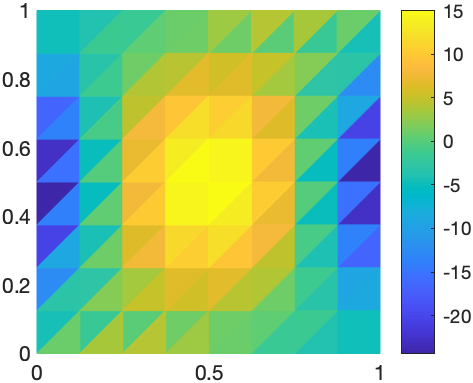
\includegraphics[width=0.7\textwidth]{img/numericalU.png} %插入图片,[]中设置图片大小,{}中是图片文件名
    \caption{数值结果} %最终文档中希望显示的图片标题
    \label{Fig.numericalU} %用于文内引用的标签
\end{figure}
收敛情况如图\ref{Fig.RateOfConvergence},可以看到基本$\mathbf{u}$和$p$都可以达到一阶收敛。
\begin{figure}[H] %H为当前位置,!htb为忽略美学标准,htbp为浮动图形
    \centering %图片居中
    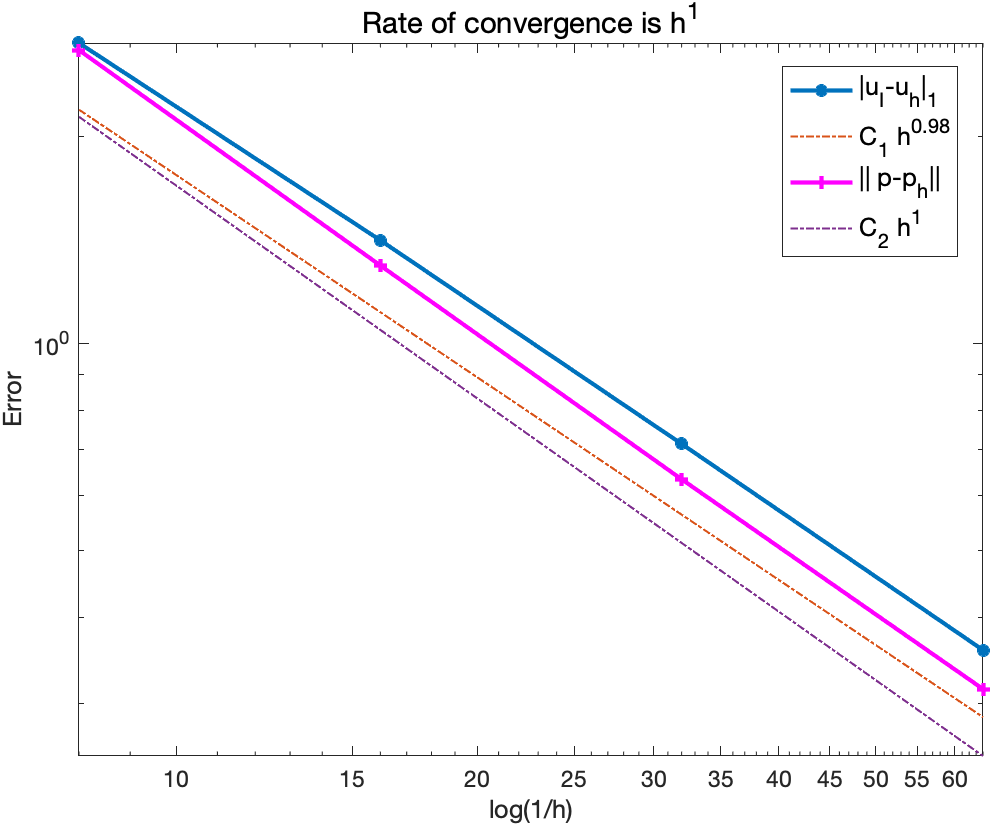
\includegraphics[width=0.7\textwidth]{img/RateOfConvergence.png} %插入图片,[]中设置图片大小,{}中是图片文件名
    \caption{收敛阶} %最终文档中希望显示的图片标题
    \label{Fig.RateOfConvergence} %用于文内引用的标签
\end{figure}

\subsection{程序清单}
\begin{itemize}
    \item \mcode{StokesCRP0.mxl} 
    
    实时脚本,带入实例计算,
    求解Stokes方程,观察数值结果及收敛阶情况。
    
    \item \mcode{JinJinStokesCRP0.m} 
    
    用CRP0元求解Stokes方程,对iFEM\cite{iFEM}
    包中\mcode{StokesCRP0.m}做了部分修改,加入随机项接口$h$。
    
    \item \mcode{MyStokesData2.m} 
    
    二维Stokes方程实例方程,存储右端项函数$f$、
    $h$,Dirichlet边界函数\mcode{g_D},精确解\mcode{exactu},
    \mcode{exactp}。该程序对iFEM\cite{iFEM}
    包中\mcode{StokesData2.m}做部分修改,加入随机函数接口$h$。

    \item \mcode{gradbasis.m}
    
    返回重心坐标的梯度\mcode{Dlambda},三角形元面积\mcode{area}。
\end{itemize}

\section{Questions}
1.\mcode{JinJinStokesCRP0.m} 105行,对$p$的处理。
\begin{lstlisting}
%% Post-process ???
if length(pDof) ~= Np % p is unique up to a constant
    % impose the condition int(p)=0
    c = sum(p.*area)/sum(area);
    p = p - c;
end
\end{lstlisting}

2.\mcode{JinJinStokesCRP0.m} 246行,对于只有Dirichlet边界的情况,
对\mcode{pDOf}的处理。
\begin{lstlisting}
% modfiy pressure dof for pure Dirichlet
if isempty(Neumann)
    pDof = (1:Np-1)'; % ??
end
\end{lstlisting}

\renewcommand\refname{参考文献}
%\bibliomatter
\nocite{*} %打印全部参考文献
\printbibliography[heading=bibliography,title=参考文献]

\end{document}